\newpage
\section{}

\subsection{}
\textbf{Pure water was quasi-statically cooled from room temperature to $-5^{\circ}$C under $1$ atm pressure. Calculate the critical nucleus radius under these conditions. Assume the nucleus is spherical, the latent heat is $6$ kJ/mol, the interfacial energy between ice and water is $30$ mJ/m$^2$, and the density of ice is $1$ g/cm$^3$.}

The critical nucleus radius can be calculated using the following equation: 
\begin{align}
  \label{eq:r01}
  r^*&=\dfrac{-2\gamma}{\Delta G_v},
\end{align}
where $\gamma$ is the surface free energy, and $\Delta G_v$ is the volume free energy change. Because $\Delta G_v$ is a function of temperature:
\begin{align}
  \label{eq:deltagv}
  \Delta G_v&= \dfrac{\Delta H_f\left(T_m-T\right)}{T_m}.
\end{align}
Substituting equation \ref{eq:deltagv} in \ref{eq:r01} gives: 
\begin{align}
  \label{eq:nucleus_radius}
  r^*&=\left(\dfrac{-2\gamma T_m}{\Delta H_f}\right)\left(\dfrac{1}{T_m - T}\right),
\end{align}
where $\gamma$ is the surface free energy in J/m$^2$, $\Delta H_f$ is the the latent heat of fusion in J/m$^3$, $T_m$ is the melting temperature in K and $T$ is the transformation temperature in K \citep[p.~346-347]{callister2010materials}.

Because the latent heat provided in the problem is given in kJ/mol, it is necessary to convert to J/m$^3$ for the calculation. Using the density of ice and the molar mass for water, 18.01528 g/mol:
\begin{align}
  \begin{split}
    \left(\dfrac{6000\text{ J}}{\text{mol}}\right)\left(\dfrac{1\text{ mol}}{18.01528\text{ g}}\right)\left(\dfrac{1\text{ g}}{\text{cm}^3}\right)\left(\dfrac{100\text{ cm}}{1\text{ m}}\right)^3&=333050610.370752 \text{ J/m}^3 \\
  &\approx 3.33\times10^{-8} \text{ J/m}^3
  \end{split}
  \label{eq:deltaH_calculation}
\end{align}

Using equation \ref{eq:nucleus_radius}, the critical nucleus radius can be calculated:
\begin{align}
  \label{eq:radius}
  \begin{split}
    r^*&=\left(\dfrac{-2*0.03*273}{-333050610.370752}\right)\left(\dfrac{1}{273-268}\right)=9.836342879999998\times 10^{-9}\text{ m} \\ 
    r^*&\approx 9.84\times 10^{-9} \text{ m}
  \end{split}
\end{align}

\begin{mdframed}
The critical nucleus radius for water quasi-statically cooled from room temperature to $-5^{\circ}$ is 9.84 nm.
\end{mdframed}

%\shnote{tengo que arreglar lo del calculo, porque el calor latente deberia de estar en kj/m3 y yo lo tengo en J/m2 asi que algo tengo que hacerle con la densidad pero no se que? :c ya se, las dimensionales no estan bien, eso es lo que tengo que arreglar}

\subsection{}
\textbf{Explain how the critical nucleus radius changes if the pure water is
further cooled, including the reason.}

To visualize the changes of the radius with further cooling water, the critical radius was calculated for different cooling temperatures, with a range of cooling temperatures of $-5$ to $-200^{\circ}$C, using equation \ref{eq:nucleus_radius}. The results were plotted in a graph, which is shown in figure \ref{fig:critical_radius}:

\begin{figure}[h]
    \centering
    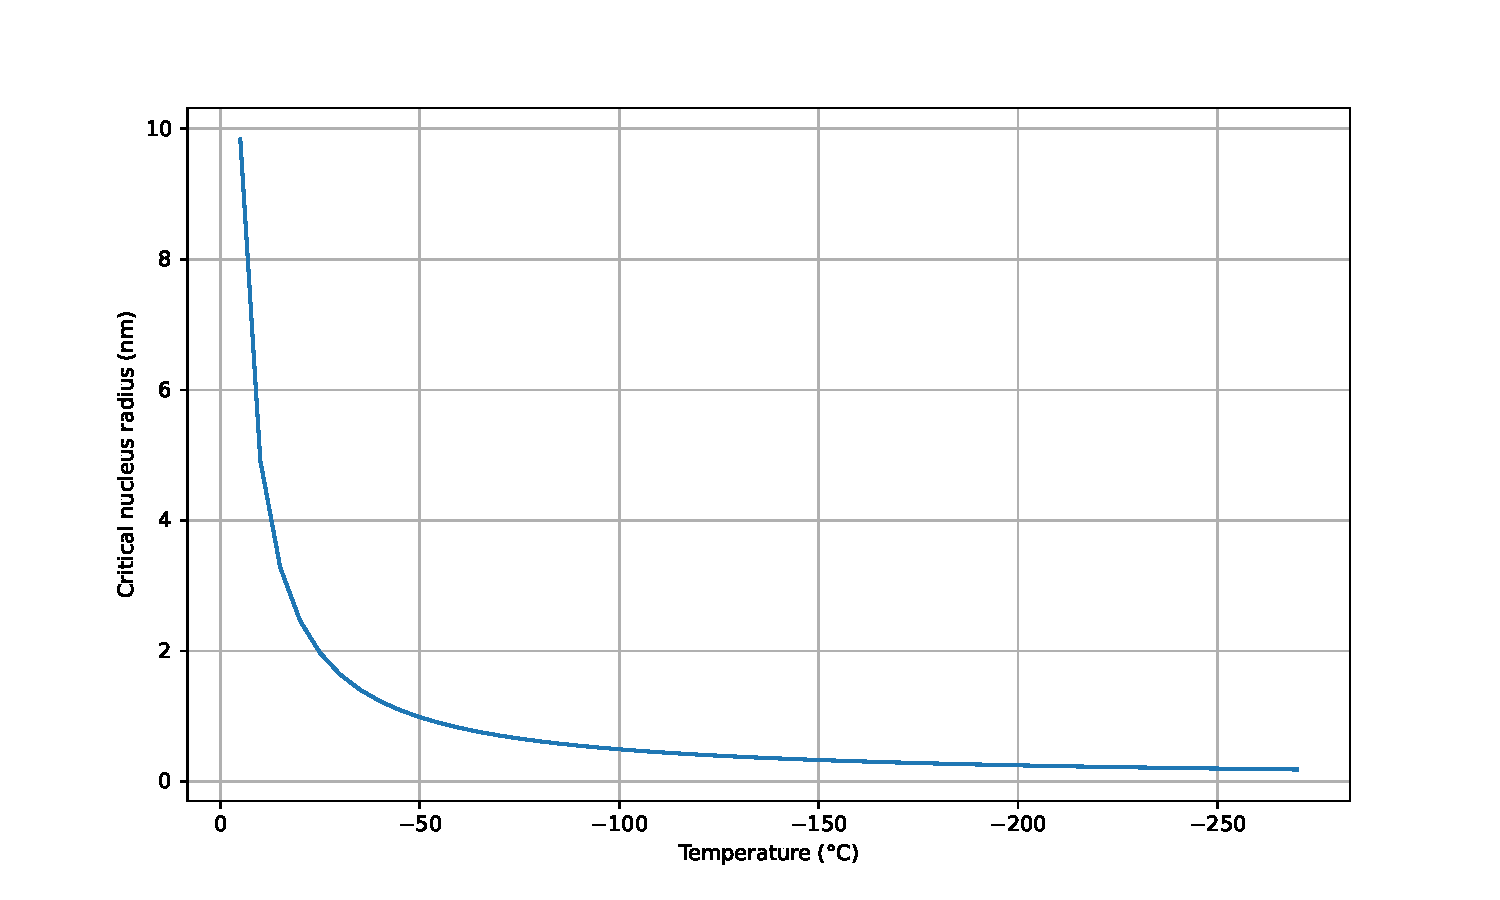
\includegraphics[width=1\textwidth]{graficas/critical_radius.pdf}
    \caption{Critical nucleus radius as a function of temperature for water cooled in a range of temperature from $-5$ to $-200^{\circ}$ C. \\
    \textit{Source: Visualization by the author (code available at \citet{mygit})}}
    \label{fig:critical_radius}
\end{figure}

\shnote{me falta explicar por que el radio cambia de esta manera}